\documentclass[../main.tex]{subfiles}
\begin{document}

In this appendix two \gls{cm} samples (refered to as ``scan0'' and ``scan3'',
matching the naming in figure \ref{fig:inference-comparison})
are displayed in the plain reflectance \gls{rcm}
and fluorescence \gls{fcm} modes, the digitally stained version using
\cite{Gareau2009} transformation and the stained version using the Unet-like
model with the 3 inference methods compared in \ref{sec:experiments-inference}. 
The reduction of the tiling artifacts using the diffent inference methods
is notable.

\newpage

\begin{figure}[H]
\centering
\begin{subfigure}{\textwidth}
\centering
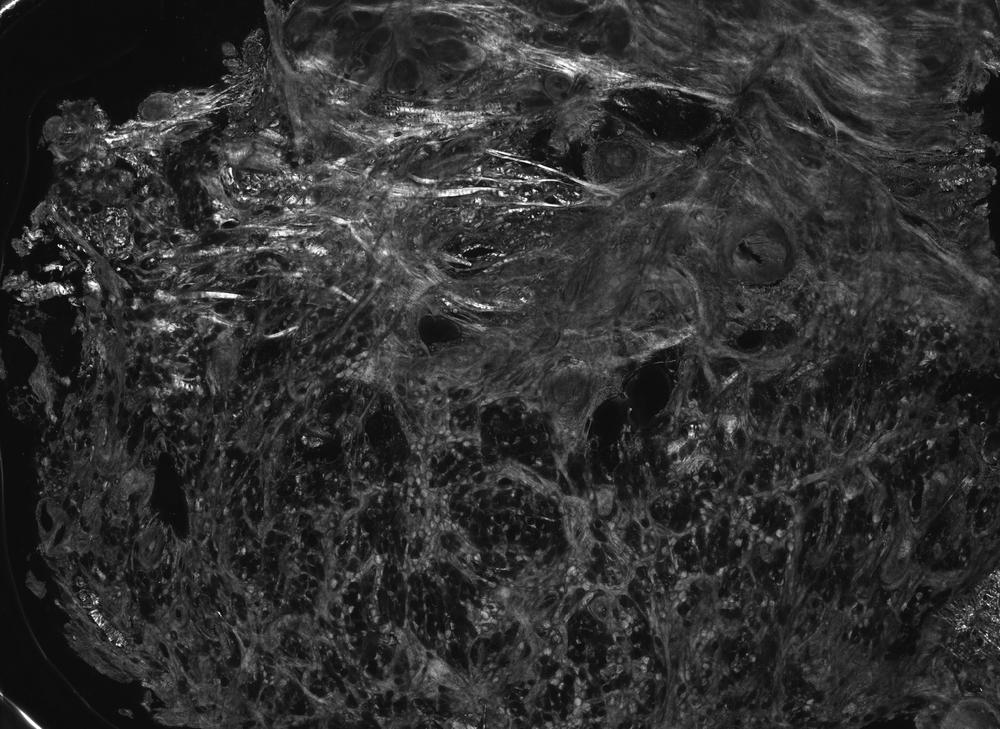
\includegraphics[width=0.9\linewidth]{scan0_R-thumbnail}
\caption{Reflectance mode.}
\label{fig:inference-comparison-scan0-R}
\end{subfigure}
\begin{subfigure}{\textwidth}
\centering
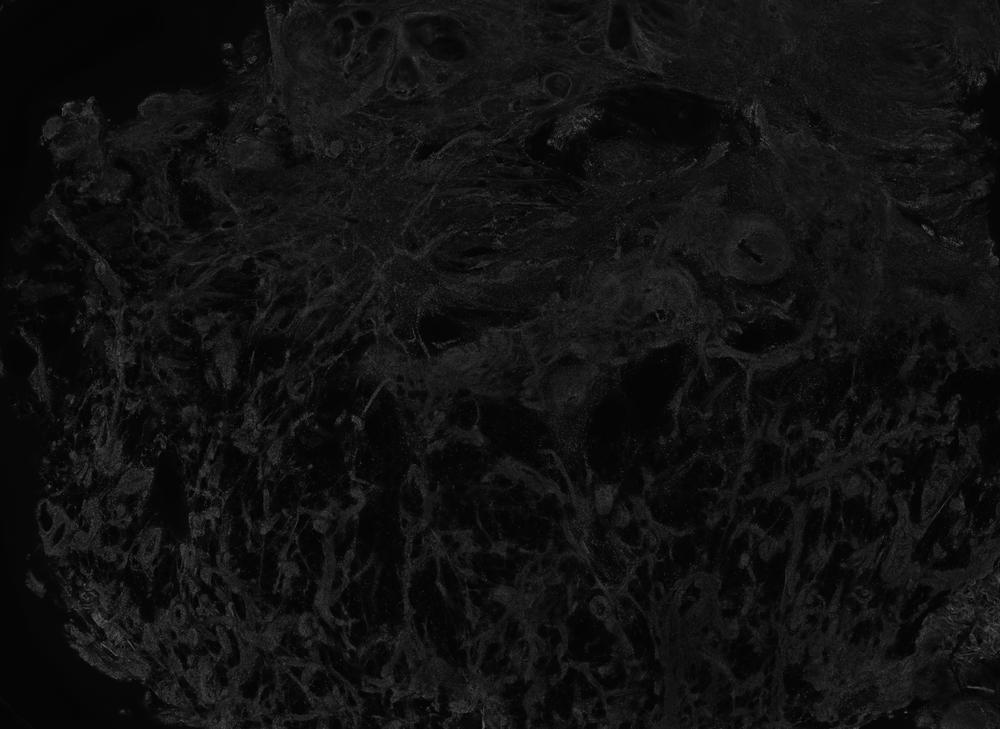
\includegraphics[width=0.9\linewidth]{scan0_F-thumbnail}
\caption{Fluorescence mode.}
\label{fig:inference-comparison-scan0-F}
\end{subfigure}
\caption{``scan0'' whole slide CM sample.}
\end{figure}

\begin{figure}[H]
\centering
\begin{subfigure}{\textwidth}
\centering
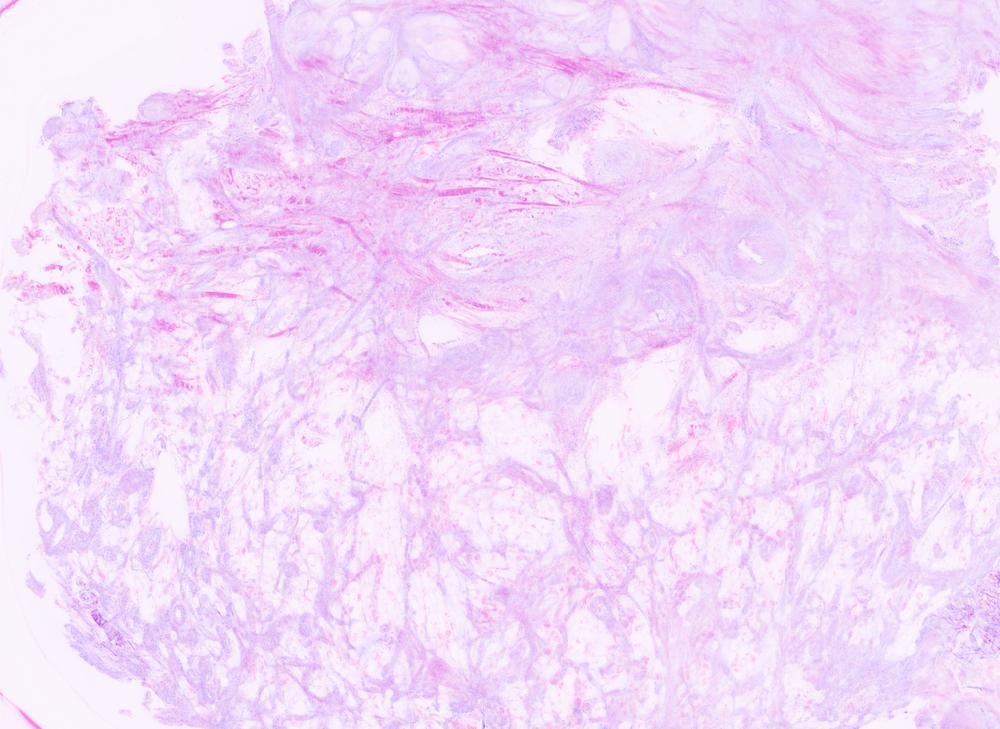
\includegraphics[width=0.9\linewidth]{scan0_linear-thumbnail}
\caption{Digitally stained slide using \cite{Gareau2009} method.}
\label{fig:inference-comparison-scan0-linear}
\end{subfigure}
\begin{subfigure}{\textwidth}
\centering
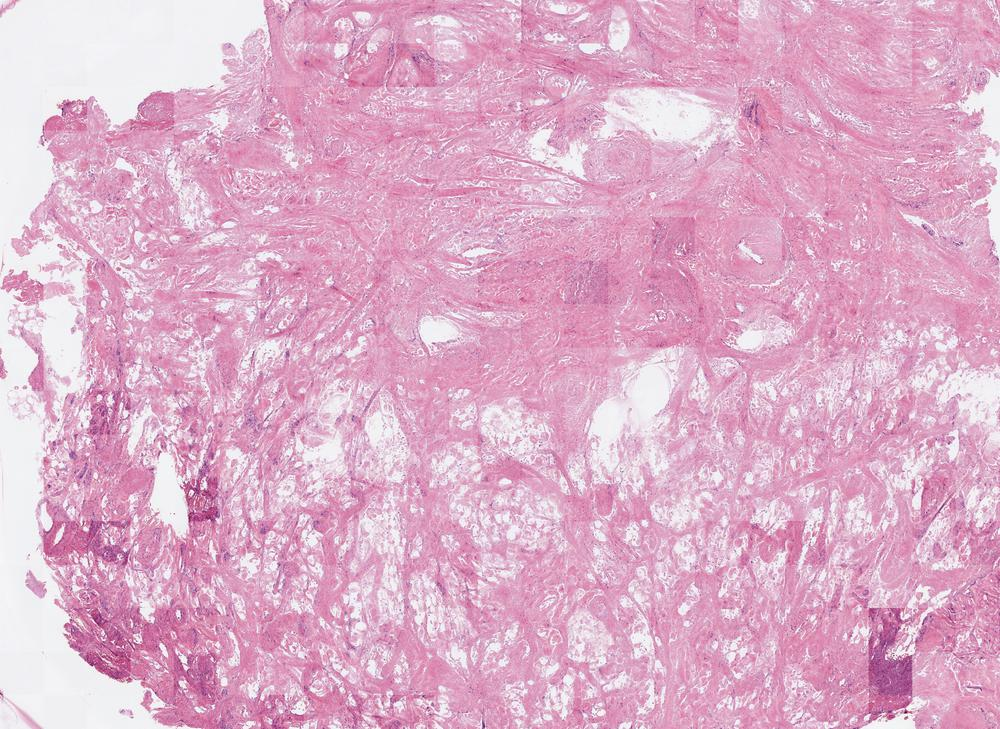
\includegraphics[width=0.9\linewidth]{scan0_independent-thumbnail}
\caption{Tile-by-tile independent inference.}
\label{fig:inference-comparison-scan0-independent}
\end{subfigure}
\end{figure}%
\begin{figure}[H]\ContinuedFloat
\centering
\begin{subfigure}{\textwidth}
\centering
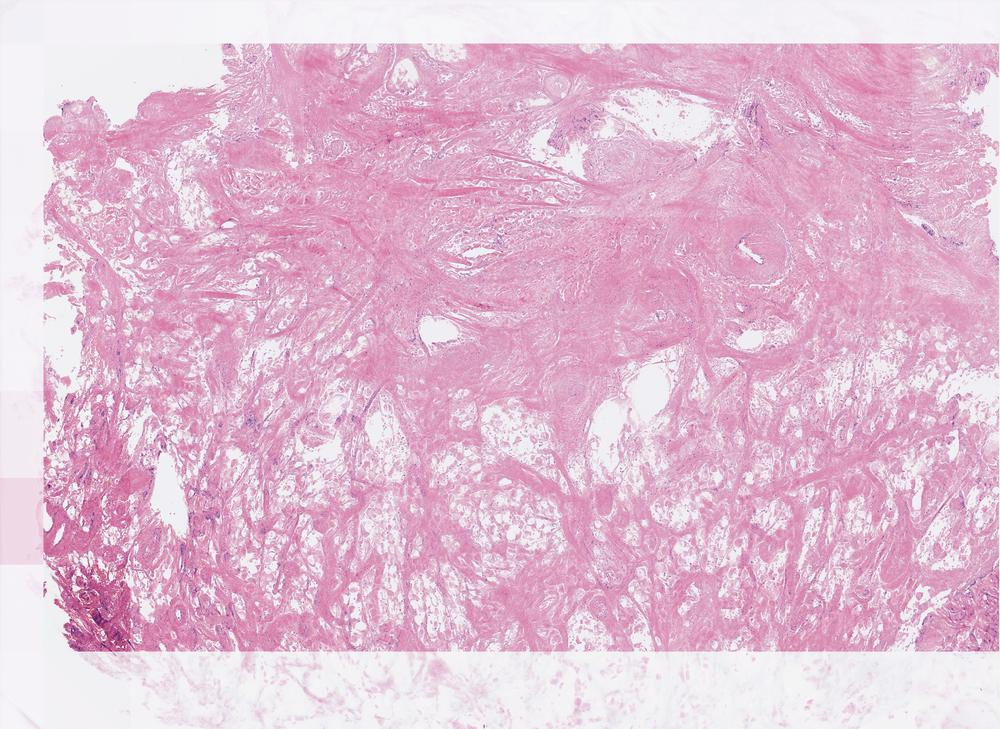
\includegraphics[width=0.9\linewidth]{scan0_no-overlap-thumbnail}
\caption{Tile-by-tile non-overlapping output inference.}
\label{fig:inference-comparison-scan0-no-overlap}
\end{subfigure}
\begin{subfigure}{\textwidth}
\centering
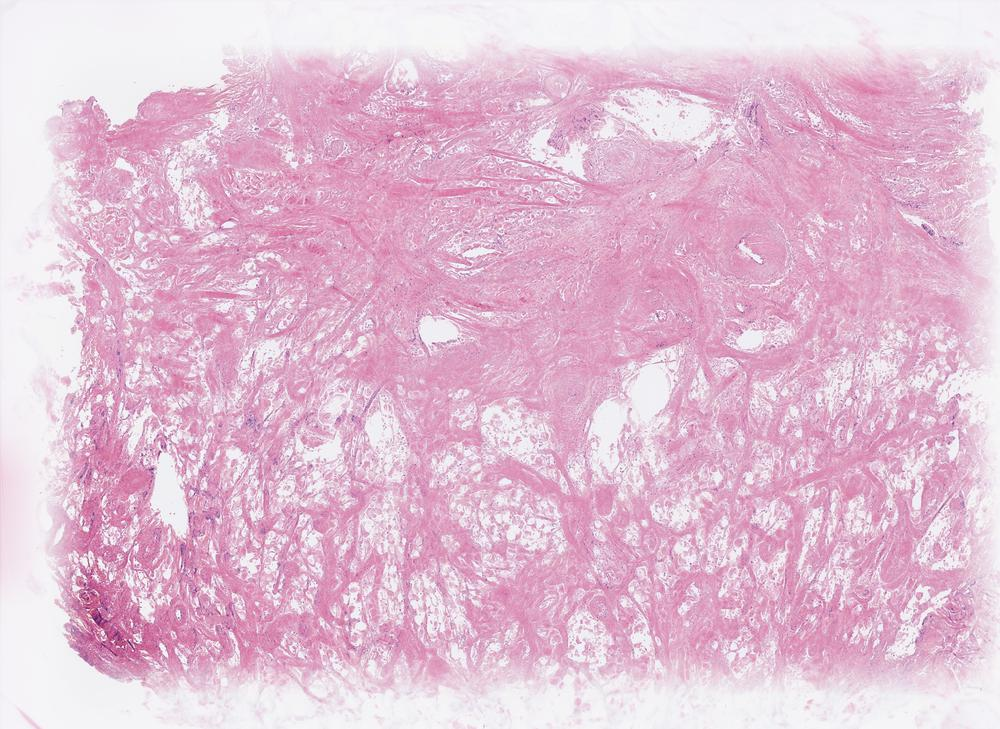
\includegraphics[width=0.9\linewidth]{scan0_pyramid-thumbnail}
\caption{Inference method based on \cite{Bel2019}.}
\label{fig:inference-comparison-scan0-pyramid}
\end{subfigure}
\caption{``scan0'' whole slide sample transformed using different inference
methods.}
\label{fig:inference-comparison-scan0}
\end{figure}

\begin{figure}[H]
\centering
\begin{subfigure}{\textwidth}
\centering
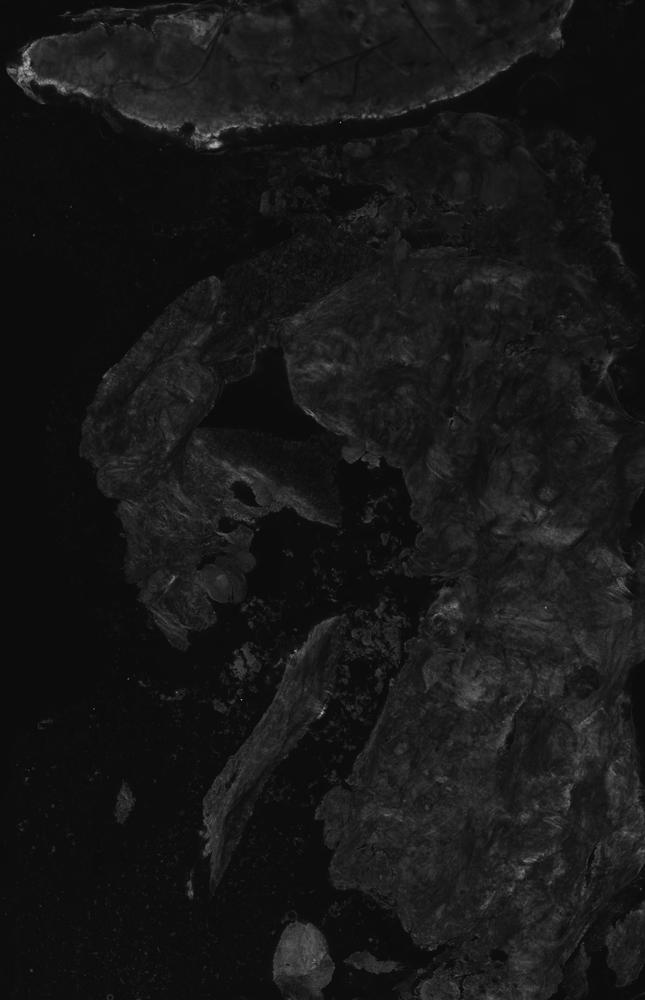
\includegraphics[width=0.9\linewidth]{scan3_R-thumbnail}
\caption{Reflectance mode.}
\label{fig:inference-comparison-scan3-R}
\end{subfigure}
\end{figure}%
\begin{figure}[H]\ContinuedFloat
\centering
\begin{subfigure}{\textwidth}
\centering
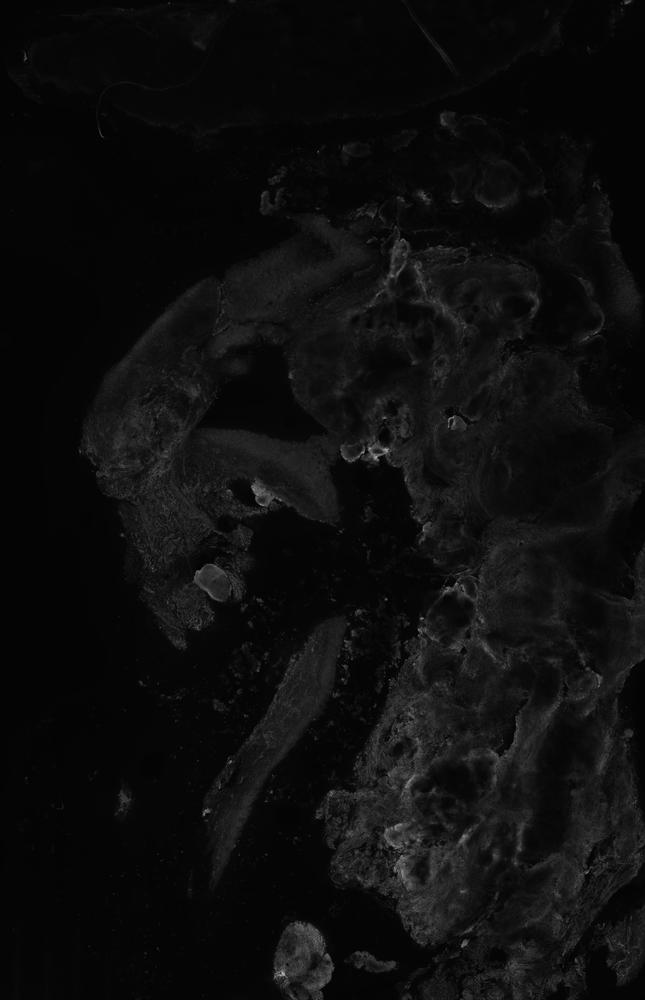
\includegraphics[width=0.9\linewidth]{scan3_F-thumbnail}
\caption{Fluorescence mode.}
\label{fig:inference-comparison-scan3-F}
\end{subfigure}
\caption{``scan3'' whole slide CM sample.}
\end{figure}

\begin{figure}[H]
\centering
\begin{subfigure}{\textwidth}
\centering
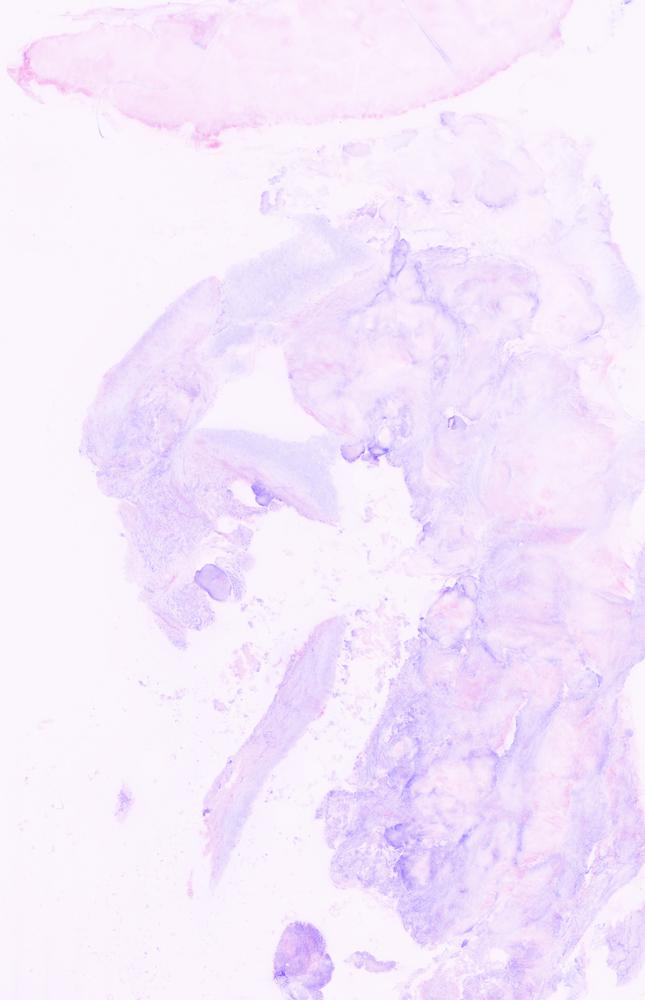
\includegraphics[width=0.9\linewidth]{scan3_linear-thumbnail}
\caption{Digitally stained slide using \cite{Gareau2009} method.}
\label{fig:inference-comparison-scan3-linear}
\end{subfigure}
\end{figure}%
\begin{figure}[H]\ContinuedFloat
\centering
\begin{subfigure}{\textwidth}
\centering
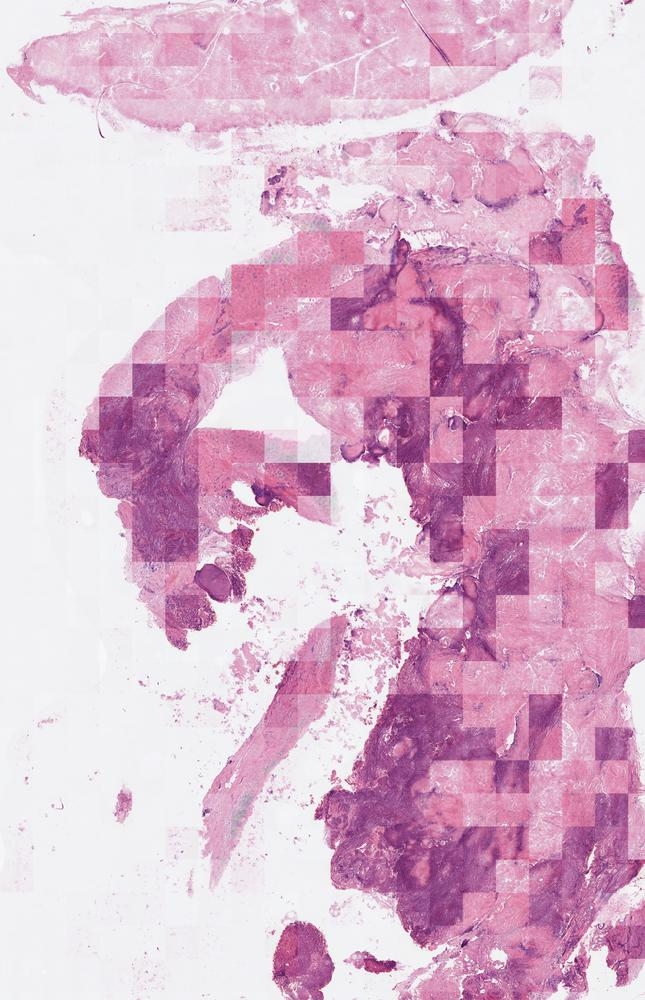
\includegraphics[width=0.9\linewidth]{scan3_independent-thumbnail}
\caption{Tile-by-tile independent inference.}
\label{fig:inference-comparison-scan3-independent}
\end{subfigure}
\end{figure}%
\begin{figure}[H]\ContinuedFloat
\centering
\begin{subfigure}{\textwidth}
\centering
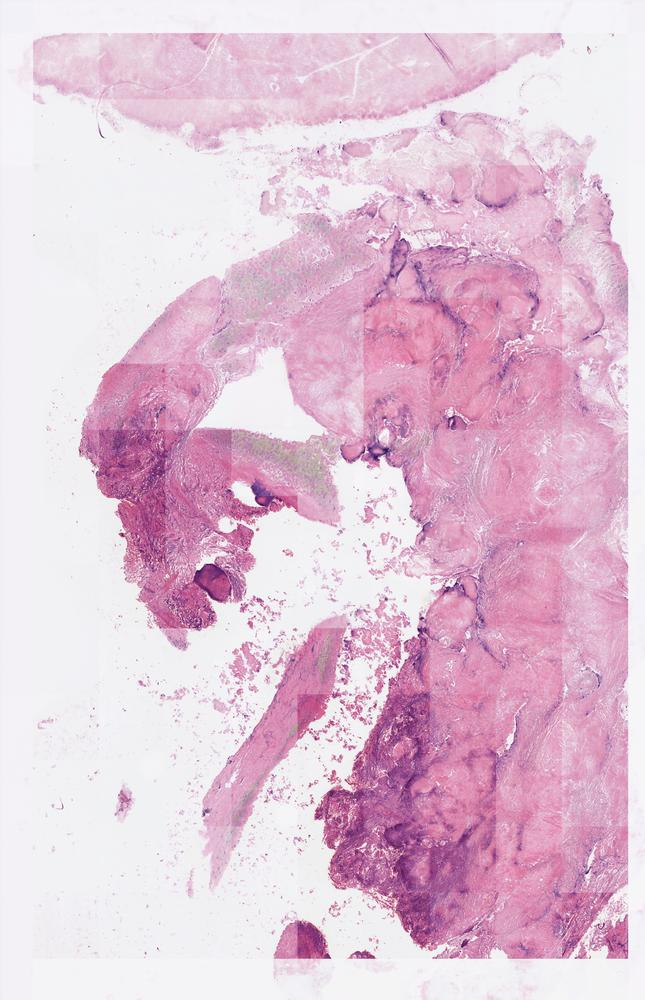
\includegraphics[width=0.9\linewidth]{scan3_no-overlap-thumbnail}
\caption{Tile-by-tile non-overlapping output inference.}
\label{fig:inference-comparison-scan3-no-overlap}
\end{subfigure}
\end{figure}%
\begin{figure}[H]\ContinuedFloat
\centering
\begin{subfigure}{\textwidth}
\centering
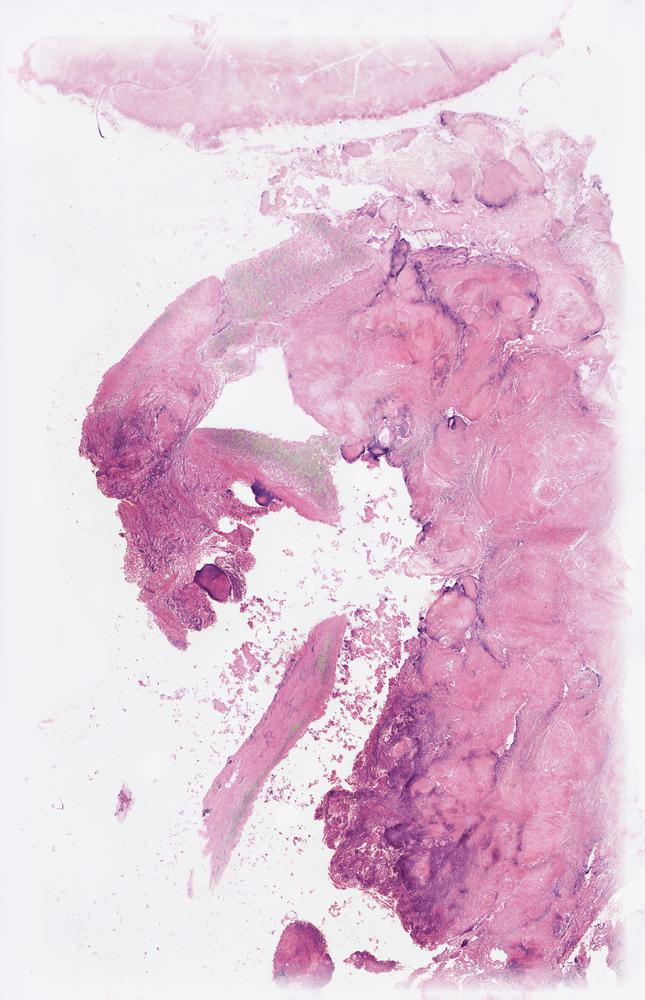
\includegraphics[width=0.9\linewidth]{scan3_pyramid-thumbnail}
\caption{Inference method based on \cite{Bel2019}.}
\label{fig:inference-comparison-scan3-pyramid}
\end{subfigure}
\caption{``scan3'' whole slide sample transformed using different inference
methods.}
\label{fig:inference-comparison-scan3}
\end{figure}

\end{document}
